\setcounter{page}{1}

% acronyms
\newacronym{api}{API}{application programming interface}
\newacronym{asic}{ASIC}{application-specific integrated circuit}
\newacronym{ast}{AST}{abstract syntax tree}
\newacronym{dsl}{DSL}{domain-specific language}
\newacronym{fpga}{FPGA}{field-programmable gate array}
\newacronym{fsm}{FSM}{finite state machine}
\newacronym{ide}{IDE}{integrated development environment}
\newacronym{ir}{IR}{intermediate representation}
\newacronym{llvm}{LLVM}{Low-Level Virtual Machine}
\newacronym{lsp}{LSP}{Language Server Protocol}
\newacronym{lto}{LTO}{link-time optimization}
\newacronym{onf}{ONF}{Open Networking Foundation}
\newacronym{p4}{P4}{Programming Protocol-independent Packet Processors}
\newacronym{repl}{REPL}{read-eval-print loop}
\newacronym{sdn}{SDN}{software-defined networking}
\newacronym{xml}{XML}{eXtensible Markup Language}
\newacronym{yacc}{YACC}{Yet Another Compiler-Compiler}
\newcommand{\pfs}{\texorpdfstring{{P}4\textsubscript{16}}{P4 16} }

\lstdefinelanguage{p4}{
	keywords={abstract,action,apply,bit,bool,const,control,default,else,enum,
	error,extern,exit,false,header,header_union,if,in,inout,int,match_kind,
	package,parser,out,return,select,state,struct,switch,table,this,transition,
	true,tuple,type,typedef,value_set,varbit,verify,void},
	sensitive=true,
	morecomment=[l]{//},
	morecomment=[s]{/*}{*/},
	morestring=[b]",
}

% Do not forget to include Introduction
%---------------------------------------------------------------
% \chapter{Introduction}
% uncomment the following line to create an unnumbered chapter
\chapter*{Introduction}\addcontentsline{toc}{chapter}{Introduction}\markboth{Introduction}{Introduction}
%---------------------------------------------------------------

% The following environment can be used as a mini-introduction for a chapter.
% Use that any way it pleases you (or comment it out). It can contain, for
% instance, a summary of the chapter. Or, there can be a quotation.
\begin{chapterabstract}
	\dots in which we get to know the context that gave rise to the
	\acrshort{p4} language and the challenges we set out to overcome.
\end{chapterabstract}

\acrfull{p4} is a domain-specific language for programming network switches. Its
release started a shift in the field of \acrfull{sdn} which, up to that point,
relied heavily on fixed-function hardware for high-performance networking
applications. Similarly to how the C language became a de facto portable
assembler, abstracting over the details of each microprocessor, \acrshort{p4}
abstracts over the details of network processors by presenting a deeply
customizable interface shared by networking software and hardware alike.

Unlike previous approaches in \acrshort{sdn}, \acrshort{p4} does not have
built-in support for common network protocols like TCP, IP, or Ethernet.
Instead, it provides protocol-independent constructs that users can leverage in
order to define arbitrary protocols and instruct a flexible network switch on
how to handle them. This programmability lets a network engineer specify the
configuration and packet processing steps of a router architecture independently
of the underlying machinery.

\todo[inline]{we need a data/control plane description/intro}
% data plane\footnote{Also known as the ``forwarding plane."}
% A \acrshort{p4} compiler
% can then synthesize microcode for a given platform and generate library files
% for the control plane.

The newfound flexibility of network processor programming that \acrshort{p4}
enables does not get a chance to shine on traditional network hardware, which is
built for a predetermined set of protocols and processing functions. The real
power of \acrshort{p4} is unlocked by \emph{programmable} network processors,
which can be reconfigured to support novel protocols and forwarding setups. The
commercial sector answered the call for such hardware, for example in Intel's
Tofino line of
chips\footnote{\url{https://www.intel.com/content/www/us/en/products/network-io/programmable-ethernet-switch.html}}.

\acrshort{p4} became wildly popular in \acrshort{sdn} since its introduction in
2014\cite{p4original}, sparking both research and commercial applications. Three
years later, \acrshort{p4} underwent a major redesign\cite{p416}, which
simplified the syntax and removed special-purpose language constructs in favour
of more general solutions\footnote{Specifically, features like counters and
checksum units were replaced by \extern{}s, a universal construct for specifying
additional hardware capabilities not explicitly covered by the core syntax. The
language shrank from over 70 to less than 40
keywords\cite{p416:v1:spec:comparison}.}. The redesigned language is known as
\pfs\cite{p416:v123:spec} and its specification has since received more
incremental updates.

%-------------------------------%
\section*{A Growing Community}
%-------------------------------%

\acrshort{p4} gave rise to a varied ecosystem of commercial offerings of both
hardware and software. It spawned several academic projects that investigated
its semantics\cite{doenges2021petr4}, allocation to heterogeneous
hardware\cite{sultana2021flightplan}, open-source network
testing\cite{antichi2014osnt}, and sketch-based
monitoring\cite{namkung2022sketchlib}, among many
others\cite{liatifis2023advancingp4survey}. The \acrfull{onf}
maintains\cite{p4onf} an open-source reference implementation of a
\pfs\footnote{Although primarily developed for \pfs since the revision of the
language, it is also capable of migrating P4\textsubscript{14} programs to \pfs
or directly compiling them.} compiler frontend and mid\-end, along with several
backends:

\begin{description}
	\item[p4c-bm2-ss] Targets a sample software switch for testing purposes.
	\item[p4c-dpdk] Targets the DPDK software switch (SWX) pipeline\cite{dpdkDPDKRelease}.
	\item[p4c-ebpf] Generates C code which can be compiled to eBPF
		and then loaded in the Linux kernel.
	\item[p4test] A source-to-source P4 translator for testing, learning compiler
		internals and debugging.
	\item[p4c-graphs] Generates visual representations of P4 programs.
	\item[p4c-ubpf] Generates eBPF code that runs in user-space.
	\item[p4tools] A platform for P4 test utilities, includes a test-case
		generator for P4 programs.
\end{description}

All of these components are open source. The frontend and mid\-end of the
reference compiler provide a foundation for hardware vendors to support
\acrshort{p4} in their products and serve the community in resolving
discrepancies between commercial compilers and the language specification.

Despite this growth, \acrshort{p4} has only mediocre support for real-time
feedback to the programmer -- the vast majority of open and commercial tools
rely on compiler output to provide semantic insight into a P4
program\cite{p4insight}, or, as evidenced by the open backends, are parts of the
compiler proper. This is a problem, because the compiler was not designed for
interactive use. Compilations of complex programs can take over an hour to
complete. Long feedback loops hamper development. What's more, information
provided by the compiler frontend is very limited -- the compiler typically
reports at most one error message with very little (if any) explanation. The
lack of an integration between the compiler and development environments is an
obstacle to new users and a neglected area of \acrshort{p4} developer
experience. Even an ergonomic presentation of error and warning messages would
be a large improvement.

We can do far better, as interactive editing support for conventional
programming languages clearly demonstrates. Integrated developer environments
provide many features that \acrshort{p4} programmers can only dream of,
including autocompletion, documentation pop-ups, real-time diagnostics, code
navigation, automatic formatting, and refactoring. These features are not only
convenient, but also improve the quality of software by reducing the cognitive
load on the programmer.

%-----------------------------------------%
\section*{Language Servers to the Rescue}
%-----------------------------------------%

Over the last decade, \emph{language servers} became a popular
architecture\cite{barros2022editing} for providing semantically informed editing
features in integrated developer environments and lightweight source code
editors alike. Although examples of language server -like tools predate their
standardization\cite{bour2018merlin}, a major milestone in their development was
the introduction of the \acrfull{lsp}. The support of \acrshort{lsp} in Visual
Studio Code seeded an ever-growing environment of cross-platform tooling for a
variety of programming, configuration, specification, and markup languages.
Their success can be attributed in part to the investment by Microsoft. However,
\acrshort{lsp} as a standard has much technical merit.

Before the introduction of a common communication interface between
language-specific tooling and a given source code editor, implementors had to
create and maintain extensions for any number of different environments, often
in several programming languages. For example, take an editor plugin providing
smart completion and "go to definition" features for the Python programming
language. Suppose the author aims to extend Vim, Emacs, and IntelliJ IDEA. They
would therefore have to reimplement the given functionality in vimscript, Emacs
Lisp, and a JVM-based language. Even though recent innovations in classical text
editors\footnote{One such project is a fork and refactoring of Vi IMproved,
\emph{Neovim}: \url{https://github.com/neovim/neovim}.} have partly moved away
from using their own \acrshort{dsl}'s, the author is still burdened with three
times the implementation work, as every development environment \acrshort{api}
is different.

The solution to this problem is to split editor extensions according to the
client-server model. The major implementation work for domain-specific
functionality resides on the server side, whereas the client is only a
relatively thin wrapper that adapts a given editor's API. Implementors can build
many thin clients for different development environments that all connect to the
same \emph{language server}. \acrshort{lsp}'s raison d'être is support of this
model in Visual Studio Code.

Coden\-vy, Microsoft, and Red Hat collaborated on standardizing the protocol to
enable other tools to benefit from shared
tooling\cite{sdtimesCodenvyMicrosoft,infoworldMicrosoftbackedLanguage}.

% these comments make the section visible from the editor minimap
%-------------------%
%-------------------%
%-------------------%
%-------------------%
%-------------------%
%-------------------%
%-------------------%
%-------------------%
%-------------------%
%-------------------%
%-------------------%
\section{Outline}
%-------------------%
%-------------------%
%-------------------%
%-------------------%
%-------------------%
%-------------------%
%-------------------%
%-------------------%
%-------------------%
%-------------------%
%-------------------%
%-------------------%

\begin{enumerate}
	\item (intro) P4 information
	\item (intro) language servers, VS Code (screenshots, c++?)
	\item design: overview of the architecture, interfaces with the editor, what
		needs to be implemented
	\item subsections about problems that needed solving, but most should go
		into the design part!
	\item results, what it can do, open-source repository, performance metrics
		(aim for interactivity)
	\item conclusion, next steps
\end{enumerate}








\todo[inline]{authorship: link to GitHub, detail which non-critical parts were
implemented by a colleague}


\begin{lstlisting}[
	caption={~Useless code},
	label=list:8-6,
	captionpos=t,
	float,
	abovecaptionskip=-\medskipamount,
	belowcaptionskip=\medskipamount,
	language=C
]
	#include<stdio.h>
	#include<iostream>
	// A comment
	int main(void)
	{
		printf("Hello World\n");
		return 0;
	}
\end{lstlisting}

%%%%%%%%%%%%%%%%%%%%%%%%%%%%%%%%%
% alternative using package minted for source highlighting
% package minted requires execution with `-shell-escape'
% e.g., `xelatex -shell-escape ctufit-thesis.tex'
% \begin{listing}
% \caption{Zbytečný kód}\label{list:8-6}
% \begin{minted}{C}
%     #include<stdio.h>
%     #include<iostream>
%     // A comment
%     int main(void)
%     {
%         printf("Hello World\n");
%         return 0;
%     }
% \end{minted}
% \end{listing}
% %%%%%%%%%%%%%%%%%%%%%%%%%%%%%%%%%

\begin{table}\centering
\caption[Příklad tabulky]{~Typesetting math}\label{tab:mathematics}
\begin{tabular}{l|l|c|c}
	Typ	& Prostředí	&
		\LaTeX{}ovská zkratka	& \TeX{}ovská zkratka	\tabularnewline \hline
	Text	& \verb|math|	&
		\verb|\(...\)|	& \verb|$...$|	\tabularnewline \hline
	Displayed	& \verb|displaymath|	&
		\verb|\[...\]|	& \verb|$$...$$|	\tabularnewline
\end{tabular}
\end{table}


%---------------------------------------------------------------
\chapter{The P4 Language}
%---------------------------------------------------------------

\begin{chapterabstract}
	\dots in which we delve into the syntax and semantics of \acrshort{p4},
	explain its use cases, and discuss the differences to conventional programming
	languages.
\end{chapterabstract}

One of the original motivations behind \acrshort{p4} was the need for
restriction. While other \acrlong{dsl}s, such as Click\todo{citation}, existed
at the time, their embeddings within general-purpose programming languages made
it difficult to analyze data dependencies crucial for scheduling parallel
execution. The expressiveness of a language complicates its efficient
compilation. In the words of Robert Harper,

\begin{displayquote}
	\textit{The expressive power of a programming language arises from its
	strictures and \emph{not} from its affordances.}

	-- Robert Harper, \citedate*{pfpl1oplss2019} \cite{pfpl1oplss2019}
\end{displayquote}

Rather than embedding \acrshort{p4} in an existing language, these
considerations motivated a clean-slate design. However, to understand why is
packet processing any different from tasks suited to general-purpose programming
languages, we need to familiarise ourselves with the switching architecture.

%----------------------------%
\section{What's in a switch}
%----------------------------%

In the following text, we choose to use \emph{switch} to mean a general packet
forwarding device. Examples of switches are

A network switch
\todo[inline]{need a readable description of this \& network routing, also
citations in the text below}

Traditionally, these devices were examples of fixed-function hardware. Various
networking protocols were implemented directly in circuitry, which made them
efficient, but inflexible. It is impossible to reconfigure a fixed-function
\acrshort{asic} to process a protocol it was not explicitly designed for in
advance. If a new, backward-incompatible version of a given protocol emerges, or
if a hardware error is found in the chip, the network administrators need to
perform a costly hardware replacement in order to support, respectively
circumvent it. Moreover, fixed-function hardware design is a lengthy and
resource-intensive process. It may take several years before an updated
fixed-function chip hits the market.

The innovation of recent years is the introduction of \emph{programmable}
network processors, which can change the set of supported protocols on the fly.
These are similar to \acrshort{fpga}s in their reconfigurability, but
specialised to packet switching and routing, which makes them more efficient. A
programmable network switch has typically no prior knowledge of networking
protocols but contains efficient circuitry for parsing and pattern-matching in
order to support arbitrary\footnote{To some degree of complexity supported by
the circuit.} protocols uploaded to the chip as microcode. While programmable
networking hardware does incur a penalty for reconfigurability, when it comes to
efficiency, it sits between fixed-function devices and completely general-purpose
solutions.

Other implementations of packet switching are also common. The already mentioned
\acrlong{fpga}s can be programmed to simulate programmable or fixed-function
networking hardware, and thus allow an even higher degree of flexibility.
Naturally, \acrshort{fpga}s are less efficient than the circuits they simulate.
Finally, there are software switches, programs for widespread processor
architectures and operating systems, such as x86 and Linux. A software switch
represents the peak of flexibility, programmability, and requires no special
hardware other than what is already commonly present in conventional computers.
Purely software-based solutions cannot compete in energy efficiency with any of
the other approaches, but are often useful for testing and in small-scale
networks.

\begin{figure}[t]
	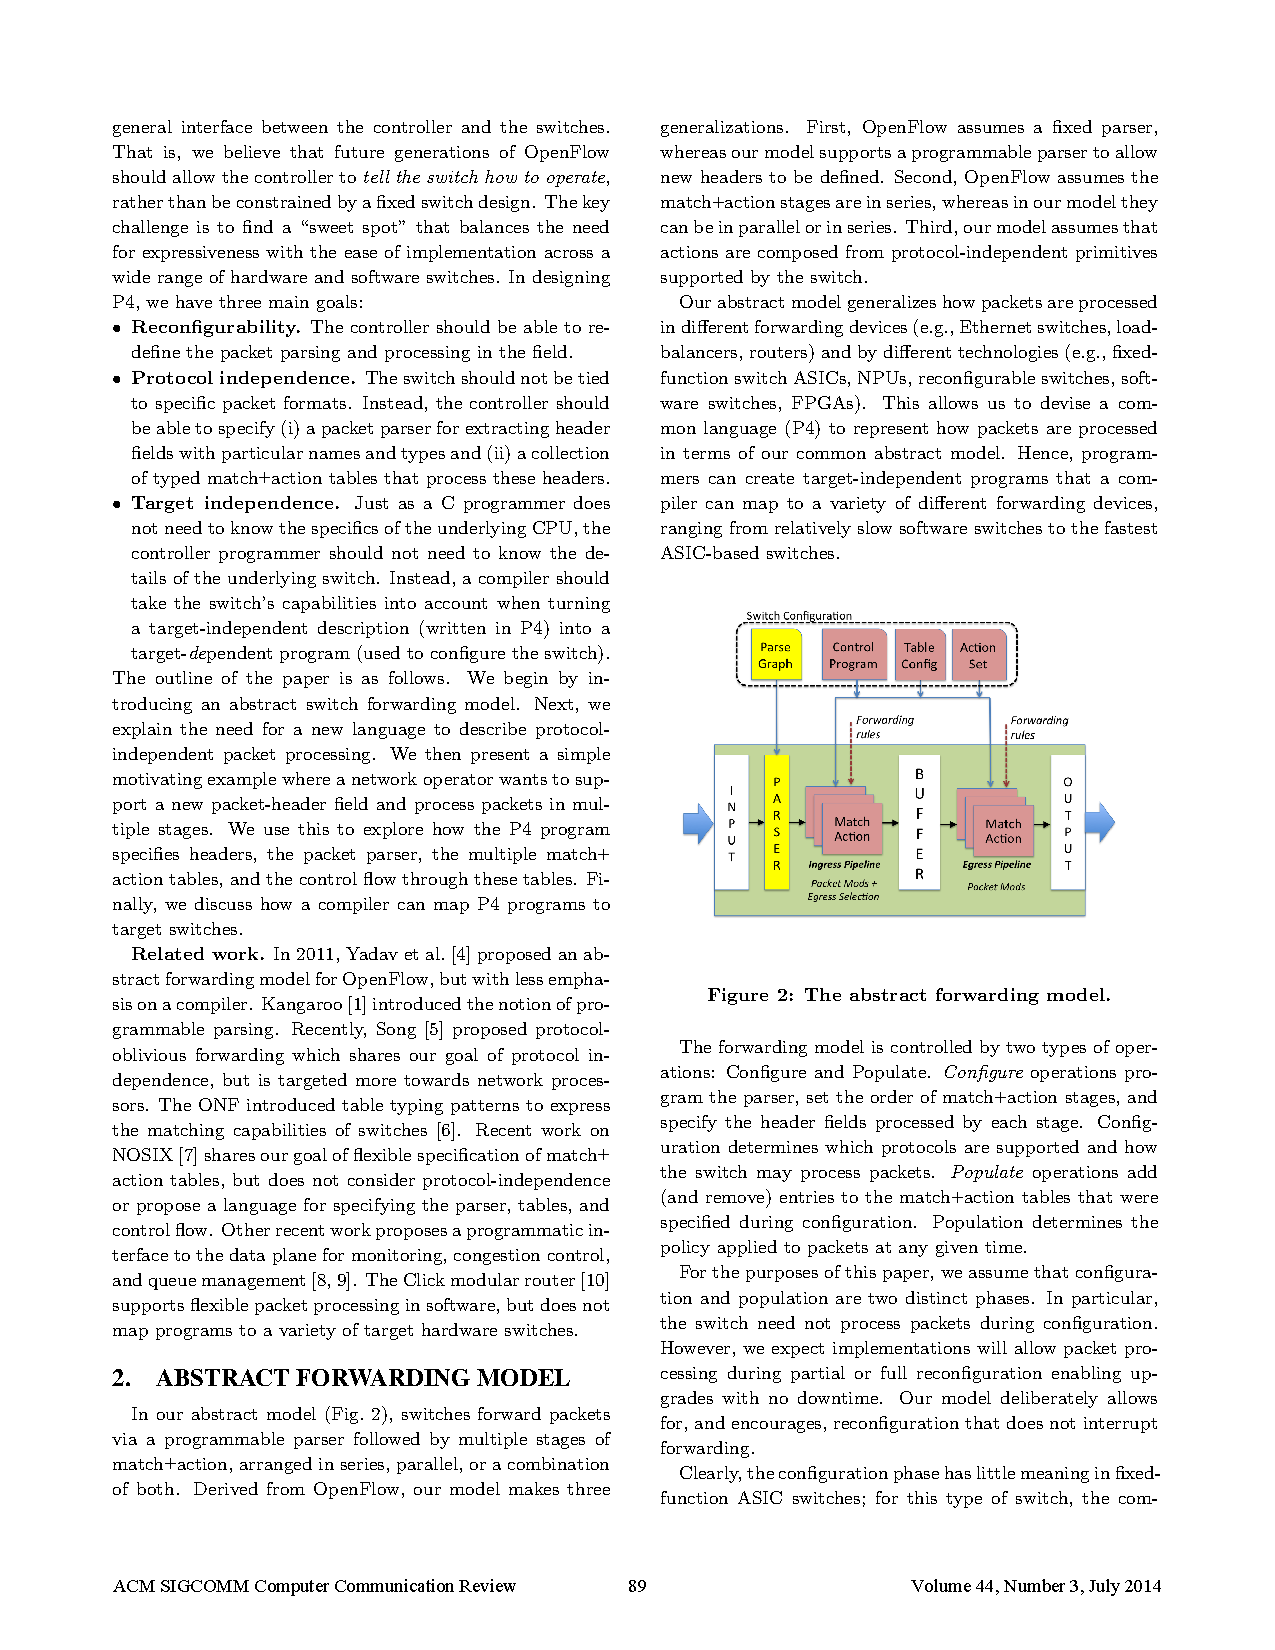
\includegraphics[
		clip,
		trim=11.5cm 12.3cm 2.7cm 10.3cm, % left bottom right top (insane, I know)
		width=1.00\textwidth
	]{resources/p4original-page-3.pdf}
	\caption{The original \acrshort{p4}\textsubscript{14} abstract forwarding
	model, taken from \cite{p4original}.}
	\label{fig:abstract-forwarding-model}
\end{figure}

To support network configurations regardless of their physical implementation,
the original \acrshort{p4} paper defines the target-independent \emph{abstract
forwarding model}, outlined in Figure~\ref{fig:abstract-forwarding-model}. This
model assumes an end-to-end pipeline split into \emph{ingress} and \emph{egress}
parts. An arriving packet is first parsed to recognize the headers present
therein. These headers then travel through the pipeline's \emph{match-action
units}. A match-action unit performs limited pattern-matching and rewriting on
the parsed packet header. This part of the pipeline is partially configured at
runtime by the control plane. Forwarding rules defined in software are uploaded
to the network device.

\todo[inline]{all this needs a much better explanation! it's crucial for
understanding the P4 way of doing things.}

The model assumes that the payload is handled separately by the device and is
not available for pattern-matching.

\todo[inline]{finish the model description, mention deparsers, explain metadata}

A lifetime may end early if the packet is dropped during processing. Dropping is
indicated by mutating metadata.

%--------------------------%
\section{The \pfs language}
%--------------------------%

\begin{figure}[t]
	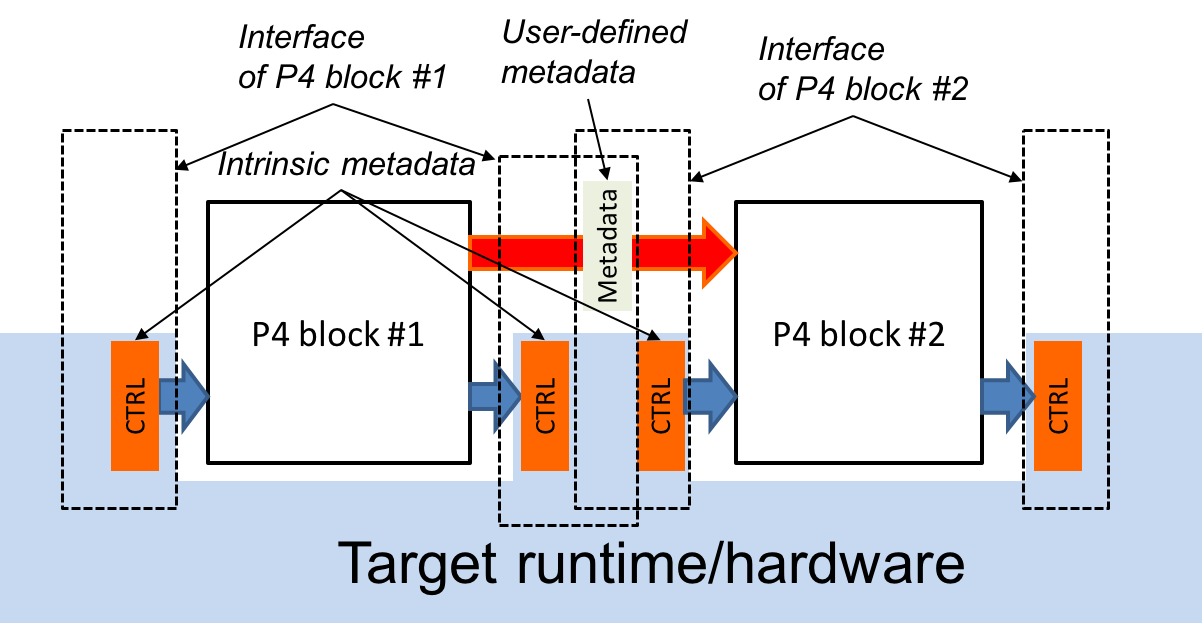
\includegraphics[width=1.00\textwidth]{resources/p4_16-architecture-model.png}

	\caption{\pfs program interfaces for an abstract architecture with two
	programmable blocks, taken from \cite{p416:v123:spec}.}
	\label{fig:arch-model}
\end{figure}

\acrshort{p4} is not a programming language for von Neumann architectures. The
abstract model assumes the target machine to be some sort of network processor
with programmable blocks embedded in a static pipeline.
Figure~\ref{fig:arch-model} illustrates such a machine and highlights the
interfaces of the \acrshort{p4} program.

A \acrshort{p4} program specifies a mapping of vectors of bits -- a bit\-vector
endomorphism. Every \acrshort{p4} program terminates; the language has no
looping constructs and no recursion, a compiler can thus determine the precise
maximum runtime of a program statically.

\todo[inline]{in discussing the subpar nature of the spec, include examples of
	mistakes.
	\href{https://p4.org/p4-spec/docs/P4-16-v-1.2.3.html\#sec-minsizeinbits}
	{compile-time size determination} mentions ``\emph{Each of these method
	calls evaluate to compile-time known values that return the minimum size in
	bits required to store the expression,}'' clearly forgetting to take the
	\texttt{maxSize*} functions into account}

\subsection{Syntax}

\todo[inline]{
	describe headers and their relation to structs, explain annotations
}

% relevant p4 spec sections

% 6.1.   Syntax and semantics
% 6.1.1. Grammar
% 6.1.2. Semantics and the P4 abstract machines
% 6.2.   Preprocessing
% 6.2.1. P4 core library
% 6.3.   Lexical constructs
% 6.3.1. Identifiers
% 6.3.2. Comments
% 6.3.3. Literal constants
% 6.4.   Naming conventions
% 6.5.   P4 programs
% 6.5.1. Scopes
% 6.5.2. Stateful elements
% 6.6.   L-values
% 6.7.   Calling convention: call by copy in/copy out
% 6.7.1. Justification
% 6.7.2. Optional parameters
% 6.8.   Name resolution
% 6.9.   Visibility

\pfs syntax is reminiscent of imperative programming languages in the C family.
It uses prefix notation for typed bindings, braces for lexical scoping blocks,
and semicolons to separate statements. However, instead of general-purpose
procedures, the top level constructs for executable code are mainly controls,
parsers, and actions. These will be explained in detail in this section.

\subsubsection*{\texttt{extern} objects and functions}

Before diving into the bulk of the syntactical forms that dominate user-written
\acrshort{p4} code, we need to introduce the general concept of
\texttt{extern}s. These special objects and functions were already present in
\acrshort{p4}\textsubscript{14} version 1.1. \pfs fully embraced these
constructs, which helped to both simplify and generalize the language.

\texttt{extern} objects and functions describe interfaces to facilities provided
by the architecture, as well as certain built-in language
constructs\todo{reference the parser declaration grammar section}. For example,
the \texttt{extern} object in Listing~\ref{lst:p4-extern-cksum} allows
\acrshort{p4} code to utilize a fixed-function checksum unit provided by the
target. The object specifies no implementation for the listed constructors and
methods.

To invoke a method of the checksum unit, the user needs first to
\emph{instantiate} the \texttt{extern} object. This syntactic form is shared
among all types with constructors: \texttt{control} blocks, \texttt{parser}s,
and \texttt{package}s\todo{describe those somewhere}. The effect of an
instantiation is to allocate the corresponding object, binding it to the
specified name.

The compiler is in charge of mapping instances of \texttt{extern}s to the target
architecture. If it does not find a mapping, either because the target does not
support the \texttt{extern} or does not have the resources to fit all its
instances, the compilation fails with an error.

\begin{lstlisting}[
	caption={~An \texttt{extern} object specifying the interface to the target's checksum unit.},
	label=lst:p4-extern-cksum,
	captionpos=t,
	tabsize=4,
	float,
	abovecaptionskip=-\medskipamount,
	belowcaptionskip=\medskipamount,
	language=c
]
extern Checksum16 {
	Checksum16();              // constructor
	void clear();              // prepare unit for computation
	void update<T>(in T data); // add data to checksum
	void remove<T>(in T data); // remove data from existing checksum
	bit<16> get(); // get the checksum for the data added since last clear
}
\end{lstlisting}

\subsubsection*{Functions and parametrized code}

Functions in \acrshort{p4} come in several flavours. The first kind is known as
\emph{function declarations} and is perhaps the closest relative of procedures
in conventional imperative programming languages. The major difference is that
all parameters to a \acrshort{p4} function need to include a \emph{direction}.

\begin{description}
	\item[parameter direction] is either \texttt{in}, \texttt{out}, or
	\texttt{inout}. \texttt{in} indicates a read-only parameter with a defined
	value, \texttt{out} indicates a read-write parameter whose value is
	initially undefined upon entering the function body, and \texttt{inout}
	indicates a read-write parameter with a defined value.
\end{description}

Only l-values\todo{what are those?} can be passed as \texttt{out} and
\texttt{inout} parameters. The execution of the function call can change the
value of an \texttt{out} or \texttt{inout} parameter's corresponding l-value.
Note that \acrshort{p4} functions can combine \texttt{out} parameters and return
values.

Parameter directions are \acrshort{p4}'s way of introducing a limited form of
references, themselves a principled approach to pointers. Parametrized
\acrshort{p4} code follows a copy in / copy out calling convention, which makes
functions easy to reason about and limits side effecting behaviour of
\texttt{extern} methods. We will discuss this later in ?\todo{reference here}

.
\todo[inline]{subsubsubsection?}

Another construct for parametrized code are \emph{parser declarations}. A
\acrshort{p4} parser describes a \acrlong{fsm} whose job is to recognize valid
packets and load their headers into the storage facilities of the target. Parser
declarations define all the states of the \acrshort{fsm}, except the implicit
built-in \texttt{accept} and \texttt{reject} states further described in the
semantics section\todo{reference here}. Each parser has to contain at least the
initial \texttt{start} state. During parsing, the parser can manipulate local
state\todo{context?} in the form of variables and \texttt{extern}
instantiations. These are defined directly in the parser declaration block,
before listing any states, meaning that the type of this local context is
statically known and independent of the state the parser may appear in at
runtime. In other words, parser declarations follow lexical scoping.

States can introduce lexically-scoped local variables, but not additional
\texttt{extern}s. Other statements like conditionals, assignments, or method
calls are also allowed. The specification explicitly points out that specific
target architectures can place restrictions on the set of constructs and
operations a programmer can use within a parser.

\pfs parser declarations unrestricted by the target architecture may appear very
similar to regular imperative code. However, the important distinction between a
parser and other function-like constructs in the \pfs language are data
extraction, pattern-matching, error handling, and state transitions.

Data extraction moves information from the input packet into memory available
for pattern-matching further down the pipeline, typically registers or similar
containers. To facilitate this operation, the \acrshort{p4} core library
contains an intrinsic\todo{established term?} \texttt{extern}\todo{we should
definitely change this and the plural into a command} definition called
\texttt{packet\_in} which represents incoming packets. This special
\texttt{extern} cannot be manually instantiated\todo{make sure we explain
instantiation prior to this. Maybe externs should be described first in the
syntax section?}, but it is instantiated implicitly for every parser
parameter\todo{arg vs param} of type \texttt{packet\_in}. This allows parser
states to invoke the methods of this \texttt{extern}, shown in
Listing~\ref{lst:p4-prsr-packet-in}.

\begin{lstlisting}[
	caption={~The intrinsic \texttt{extern} that facilitates data extraction.},
	label=lst:p4-prsr-packet-in,
	captionpos=t,
	tabsize=4,
	float,
	abovecaptionskip=-\medskipamount,
	belowcaptionskip=\medskipamount,
	language=c
]
extern packet_in {
	void extract<T>(out T headerLvalue);
	void extract<T>(out T variableSizeHeader, in bit<32> varFieldSizeBits);
	T lookahead<T>();
	bit<32> length();  // This method may be unavailable in some architectures
	void advance(bit<32> bits);
}
\end{lstlisting}

\begin{lstlisting}[
	caption={~An example of data extraction in a \pfs parser.},
	label=lst:p4-prsr-extract,
	captionpos=t,
	tabsize=4,
	float,
	abovecaptionskip=-\medskipamount,
	belowcaptionskip=\medskipamount,
	language=c
]
struct Result { Ethernet_h ethernet;  /* more fields omitted */ }
parser P(packet_in b, out Result r) {
	state start {
		b.extract(r.ethernet);
	}
}
\end{lstlisting}

An example of extraction of fixed-width data can be seen in
Listing~\ref{lst:p4-prsr-extract}.

Data extraction and computation within parser states subsumes the stateful part
of a \acrlong{fsm}. Because isolated states would not be very useful on their
own, \acrshort{p4} parsers can specify state transitions using the
\texttt{transition} statement. The target of the transition can be either given
statically or computed. A missing \texttt{transition} statement at the end of a
state block implies a transition into the \texttt{reject} state.

Another parser-specific construct facilitates the computation of transition
targets by pattern-matching on extracted data. The \texttt{select} expression
tries to match a value against a number of patterns and evaluates to a state, if
successful. Otherwise, it triggers a runtime error with code
\texttt{error.NoMatch}. The patterns of a \texttt{select} expression can contain
integer literals, bit masks, ranges, don't-care values, tuples (when matching on
multiple values simultaneously), or, on some architectures, \textit{parser value
sets} specified at runtime by the control plane.\todo{one snippet to rule them
all, one snippet to find them, one snippet to bring them all and in the \LaTeX{}
bind them.}

While error-handling already happens implicitly in \texttt{select} expressions,
the \texttt{verify} statement, defined in Listing~\ref{lst:p4-prsr-verify},
allows the programmer to ergonomically check arbitrary assertions about the
parsed data. Passing \texttt{false} as the first argument to \texttt{verify}
immediately transitions to the \texttt{reject} state, setting the parser error
to the code given as the second argument. Otherwise, execution proceeds with the
next statement.

\begin{lstlisting}[
	caption={~The interface of the \texttt{verify} built-in.},
	label=lst:p4-prsr-verify,
	captionpos=t,
	tabsize=4,
	float,
	abovecaptionskip=-\medskipamount,
	belowcaptionskip=\medskipamount,
	language=c
]
extern void verify(in bool condition, in error err);
\end{lstlisting}

\begin{figure}\centering
	\begin{tikzpicture}[
		->,
		>=stealth,
		shorten >=1pt,
		auto,
		node distance=1cm,
		semithick
	]
		\tikzstyle{every state}=[fill=white,draw=black,text=black,minimum size=2em]
		\tikzstyle{cloud}=[draw=gray!20,circle,fill=gray!10,minimum height=2em]
		\tikzstyle{rejecting}=[state,double,minimum size=2em]

		\node[state] (start) {$\text{start}$};
		\node[state, below=of start] (q2) {};
		\node[state, left=of q2] (q1) {};
		\node[state, below=of q1] (q3) {};
		\node[state, below=of q2] (q4) {};
		\node[state, right=of q4] (q5) {};
		\node[state, accepting, below=1.5cm of q4] (accept) {$\text{accept}$};
		\node[rejecting, below=1.5cm of q3] (reject) {$\text{reject}$};

		\begin{pgfonlayer}{background}
			\node[cloud,fit=(q1)(q2)(q3)(q4)(q5)(start),inner sep=2pt] (cloud) {};
		\end{pgfonlayer}

		\path
			(start) edge          (q2)
			(q1)edge              (q2)
				edge              (q3)
			(q2)edge              (q4)
			(q3)edge              (q4)
				edge              (reject)
			(q4)edge              (q5)
				edge              (accept)
			(q5)edge              (accept)
			(q5)edge [bend right] (q3);
	\end{tikzpicture}
	\caption{An abstract overview of a \acrshort{p4} parser. The states inside
	the grey circle are accessible to user code.}
	\todo[inline]{add a loop}
	\label{fig:parser-overview}
\end{figure}


\begin{lstlisting}[
	caption={~A function declaration in \pfs.},
	label=lst:p4-fun,
	captionpos=t,
	tabsize=4,
	float,
	abovecaptionskip=-\medskipamount,
	belowcaptionskip=\medskipamount,
	language=c
]
bit<32> max(in bit<32> left, in bit<32> right) {
	return (left > right) ? left : right;
}
\end{lstlisting}

\todo[inline]{subparsers, header stacks}

\todo[inline]{we should really reorganise this to use bigger headings, this way
the individual constructs are lost in the text!}

While parsers execute at the very frontier of the pipeline, the bulk of packet
processing happens in match-action units\todo{previously mentioned?}.
\acrshort{p4} has another parametrized construct for expressing entire sequences
of pattern-matching and rewriting steps: \texttt{control} blocks\todo{Add an
example control block listing}.

A control block has a name and can take type and value parameters. The body of a
control block begins with declarations of constants, variables, and
instantiations. It follows with definitions of \emph{\texttt{action}s}.

A \acrshort{p4} action\todo{example listing} is a piece of code that directly
manipulates packet headers. At a first glance, actions should be immediately
familiar to imperative programmers, since they resemble functions with no return
value. Their bodies are each comprised of a series of statements. These are
executed sequentially\footnote{At least from the perspective of the
programmer.}. There are two important restrictions on action parameter lists.

\begin{enumerate}
	\item Parameters with no direction must all come at the end of the parameter
	list. These directionless parameters indicate \emph{action
	data}\todo{explain what that is}.
	\item Action parameters cannot have \texttt{extern} types.
\end{enumerate}

The second major \acrshort{p4} construct that appears exclusively\todo{right?}
within control blocks are \emph{tables}. Whereas an action specifies the
operations performed on packet headers when pattern-matching succeeds, a table
informs a match-action unit of the target how to perform the pattern-matching
and what actions to invoke.

Functional programmers will note that tables and actions together seem like a
low-level decomposition of pattern-matching from Haskell or Scala. This is a
good analogy, except that, whereas pattern-matching constructs in a programming
language are typically fixed at compilation time, \acrshort{p4} tables are
configurable at runtime by the control plane. Furthermore, \acrshort{p4}'s
pattern-matching operates at the bit level and offers certain string-like
facilities.\todo{this whole thing should be like an aside or something}

A \texttt{table} declaration is simultaneously an instantiation in the enclosing
control block. The declaration lists various properties of the table, given as
key-value pairs. It has at least the mandatory \texttt{key} and \texttt{actions}
properties, which specify an expression used for computing the lookup key and
the set of actions the table can invoke, respectively. A table declaration can
optionally also include \texttt{default\_action} and/or \texttt{size}
properties, which specify the action invoked when no other actions
match\footnote{The \texttt{default\_action} property defaults to the built-in
\texttt{NoAction} when not specified.}, and the desired size for the table.
Compilers can choose to extend this standard set of properties with additional
target-specific key-value pairs.

The programmer can optionally declare table properties as \texttt{const}. This
keyword ensures that the control plane cannot change the property's value at
runtime. Somewhat confusingly, some properties are implicitly \texttt{const},
including the standard properties \texttt{key}, \texttt{actions}, and
\texttt{size}.

\todo[inline]{some sort of heading for keys here}

The \texttt{key} table property specifies the scrutinee of pattern-matching.
Grammatically, the key is a sequence of rows where each row contains the
expression to match on, the kind of matching to perform, and a list of
optional annotations.

The possible kinds of pattern-matching are \texttt{exact}, \texttt{ternary}, and
\texttt{lpm}, all defined as part of the \texttt{match\_kind}
enumeration\todo{is it an enum?} in the core library\todo{do we discuss that
prior to this point?}. The semantics of these options is not given, it depends
on the compiler and target architecture. Key elements can be named with optional
\texttt{@name} annotations to give them readable names in the control plane
\acrshort{api}.

The \texttt{actions} table property lists all the actions that the table can
invoke at runtime, separated by semicolons.

Regarding scoping, action names of actions in the \texttt{actions} list have to
be distinct. That is, two actions of the same name cannot appear in the
\texttt{actions} list, even if they come from different scopes and could be
disambiguated with fully qualified paths in different contexts.

An overview of the valid and illegal usages of the \texttt{actions} table
property is given in Listing~\ref{lst:p4-table-actions}. The examples highlight
the distinction of action parameters with and without direction. The
directionless parameters, also known as \emph{action data}, are used to
communicate data between the control plane and the data plane at runtime, and
therefore cannot be bound in the \acrshort{p4} program. Haskell enthusiasts may
note that the distinction between compile time and runtime -bound values is
somewhat reminiscent of second-class functions.

\begin{lstlisting}[
	caption={~Use of the \texttt{actions} table property in \pfs.},
	label=lst:p4-table-actions,
	captionpos=t,
	tabsize=4,
	float,
	abovecaptionskip=-\medskipamount,
	belowcaptionskip=\medskipamount,
	language=c
]
action a(in bit<32> x) { /* body omitted */ }
bit<32> z;
action b(inout bit<32> x, bit<8> data) { /* body omitted */ }
table t {
	actions = {
		// a;
		//  - illegal, x parameter must be bound
		a(5);  // binding a's parameter x to 5
		b(z);  // binding b's parameter x to z
		// b(z, 3);
		//      - illegal, cannot bind directionless data parameter
		// b();
		//  -- illegal, x parameter must be bound
		// a(table2.apply().hit ? 5 : 3);
		//   -------------- illegal, cannot apply a table here
	}
}
\end{lstlisting}

The \texttt{default\_action} table property specifies the action invoked when no
other actions match. The value of this property is an expression that invokes
the action in question, binding parameters with directions similarly to an
\texttt{actions} list entry. It introduces an interesting redundancy in the \pfs
language, since the programmer needs to also include the default action in the
\texttt{actions} list. Moreover, the default action and the entry in the list
have to be syntactically identical, except for the directionless parameters.
Since there is no action data for the default action at runtime, the
\texttt{default\_action} property has to specify them all.

\subsection{Semantics}

The semantics of \pfs is defined entirely in terms of abstract machines
executing imperative code. A conforming compiler is free to rewrite the \pfs
program as long as it maintains the observable behaviour of all abstract
machines involved. Unfortunately, the specification gives no formal treatment
of these machines; they are described only in natural language and pseudocode.

\todo[inline]{point out how the language tries to avoid undefined behaviour
and makes arithmetic typing rules saner and safer with no undef. behaviour}


\subsubsection*{Parser abstract machine}

A parser conceptually manipulates a \texttt{ParserModel} data structure.

\begin{lstlisting}[
	caption={~The conceptual model of the state of a \acrshort{p4} parser.},
	label=lst:p4-parser-model,
	captionpos=t,
	tabsize=4,
	float,
	abovecaptionskip=-\medskipamount,
	belowcaptionskip=\medskipamount,
	language=c
]
ParserModel {
    error       parseError;
    onPacketArrival(packet p) {
        ParserModel.parseError = error.NoError;
        goto start;
    }
}
\end{lstlisting}

The meaning of \texttt{accept} and \texttt{reject} states is
architecture-dependent. For example, a rejected packet may be dropped or
passed to the next block of the processing pipeline.

Parser transitions are analogous to \texttt{goto} statements or parameter-less
tail calls.

\subsubsection*{Calling convention}

In order to simplify reasoning about function-like constructs, \pfs follows the
\emph{call by copy in / copy out} calling convention. The specification
describes the exact steps a conforming implementation needs to go follow in
general\footnote{Compiler optimizations could, in specific cases, eliminate some
of these steps, provided prior analysis determines such optimizations correct.}
to evaluate a function call expression.

\begin{displayquote}
	\emph{\begin{enumerate}
		\item Arguments are evaluated from left to right as they appear in the
		function call expression.
		\item If a parameter has a default value and no corresponding argument
		is supplied, the default value is used as an argument.
		\item For each \texttt{out} and \texttt{inout} argument the
		corresponding l-value is saved
		(so it cannot be changed by the evaluation of the following arguments).
		This is important if the argument contains indexing operations into a
		header stack.
		\item The value of each argument is saved into a temporary.
		\item The function is invoked with the temporaries as arguments. We are
		guaranteed that the temporaries that are passed as arguments are never
		aliased to each other, so this ``generated'' function call can be
		implemented using call-by-reference if supported by the architecture.
		\item On function return, the temporaries that correspond to
		\texttt{out} or
		\texttt{inout} arguments are copied in order from left to right into the l-values
		saved in Step 3.
	\end{enumerate}}

	-- \citetitle{p416:v123:spec} \cite{p416:v123:spec}
\end{displayquote}

The calling convention gives function calls\todo{I really need some sort of
universal definition of function-like constructs in p4 that I stick to
throughout the text} a semantics that ensures arguments cannot alias one another
and impure functions cannot hold references to \acrshort{p4} code. This design
is ultimately motivated by the need to control the side effects of
\texttt{extern} functions and methods, which are arbitrarily powerful. The copy
in / copy out calling convention lets compilers reason about programs in the
presence of \texttt{extern}s.

\subsubsection*{Control blocks}

Invoking actions: actions can be invoked either implicitly or explicitly.
Implicit invocations come from tables during match-action processing. Explicit
invocations are calls from \texttt{control} blocks or other \texttt{action}s. In
the explicit invocation case, directionless parameters follow \texttt{in}
parameter semantics.

%--------------------------------------%
\chapter{Language Server Architecture}
%--------------------------------------%

Language servers have a lot in common with compilers. Like compilers, they have
to build up a semantic model of a program and provide useful diagnostics for
invalid or suspicious input along the way. Unlike a compiler, a language server
needs to maintain the semantic model over the course of an editing session.
Rather than operating in batch mode, a language server runs continuously and is
expected to provide feedback within milliseconds.

However, language servers need neither to produce compilation artifacts nor to
optimise the programs they process. Instead, they are effectively
special-purpose query engines. Their output is a data structure optimised for
fast querying, such as finding references, definitions, or providing
context-sensitive completion suggestions. From that point of view, it could seem
like a language server is merely a compiler frontend\todo{decide on \& unify
"frontend" vs "front-end" (back, mid, \dots)} with very little backend logic.
Unfortunately, this is not the case.

The requirement for real-time feedback to the developer is the primary
constraint on a language server's design. For all but the most basic languages
and features, instant feedback requires an incremental computation approach and
management of state that persists across updates to source files. The second
most important consideration, and one to a large extent not shared with
compilers, is resilience to errors. While a compiler generally expects
well-formed input, a language server deals with all sorts of intermediate states
of a document, including files with many syntactic errors, invalid encodings, or
unsaved buffers outside the filesystem.

To make matters worse, while compiler frontend implementations are often guided
by a language specification\footnote{Even if, usually, an informal one.}, the
space of invalid programs is unconstrained. Developers of language servers have
to guess what intermediate states a program goes through during development and
how to respond to them. Generating meaningful semantic models from invalid input
is a challenging task, but doing so is often crucial for developers. For
example, smart auto-completion in statically typed languages is expected to
provide type-correct suggestions, even as the document being edited is
type-incorrect, and often semantically or even syntactically invalid.

In this chapter, we explore the status quo of language servers, how they differ
from conventional batch-processing compilers, how this gap may narrow in the
future, and what makes building interactive language tooling difficult.

%----------------------------------------%
\section{The fruits of semantic support}
%----------------------------------------%

\todo[inline]{
	should cover LSP ``language features'' section, current tooling, show
	especially limitations of current tools with invalid input, guessing,
	complex situations (rust-analyzer failing to infer types rustc knows about),
	etc
}

The largest language servers conforming to \acrshort{lsp} offer a wide variety
of features. The vast majority of the \acrshort{api} surface is optional,
however. Upon establishing a connection, the client and server exchange
information about their respective capabilities, establishing a subset of
\acrshort{lsp} they both support.

The functionality of \acrshort{lsp} comes in two main flavours: code
comprehension and coding features. The former subsumes utilities which ease
reading and navigating through code, such as Hover (where the editor displays
details about an object under the pointer), Go to Definition, Find References,
etc. Utilities like diagnostics, auto-completion, or code actions are more
relevant to the programmer at the time they are authoring code and belong in the
latter category.

Next, we will delve into both categories and take a closer look at what they
offer.


\subsection{Code comprehension in \acrshort{lsp}}

\todo[inline]{this is lsp 3.17}

\newcommand{\org}{\pdftooltip{(original)}{This request was present in the
original LSP specification.}}

Code comprehension functionality takes up the majority of \acrshort{lsp}'s
\acrshort{api} surface and has been growing during the protocol's evolution. The
central features, already present in the initial specification of the protocol,
are Go to Definition, Find References, Document Highlight, Document Link, Hover,
Code Lens, and Document Symbols\todo{examples for everything, including a
screenshot from Neovim or something that's not VS Code. Don't forget to add
Haskell evaluation code lenses.}.

\begin{figure}[h]
	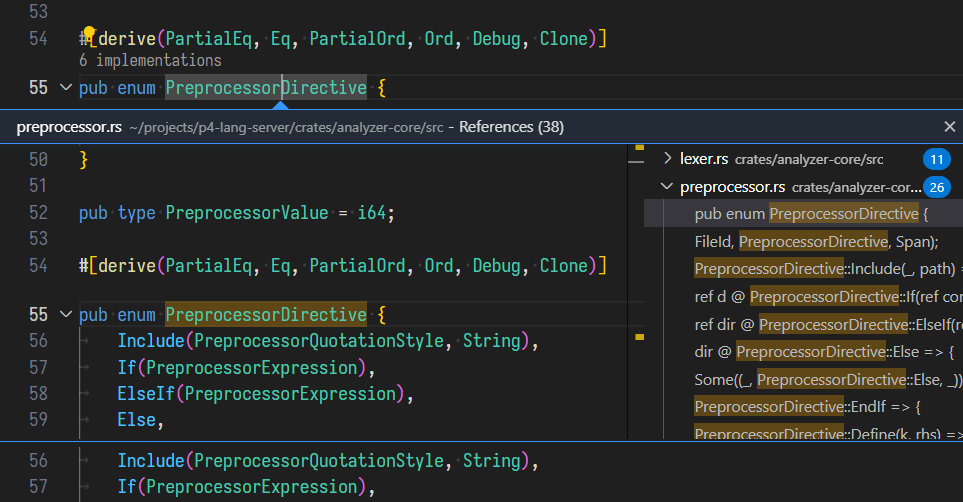
\includegraphics[width=1.00\textwidth]{resources/code_find_references.png}
	\caption{Find References in Visual Studio Code via rust-analyzer.}
\end{figure}

Go to Definition and Find References are
present in some of the oldest code comprehension tools, dating back at least to
the Unix utility \texttt{ctags}\cite{exuberant_ctags}. These let the editor jump
from a symbol's use-site to its definition and vice versa, just as their names
imply. \acrshort{lsp}'s Document Highlight request does not provide syntax
highlighting, rather, it serves to visually assist the programmer with locating
references of a given symbol without having to explicitly invoke the Find
References feature. Document Highlight could be merged with Find References
functionality, but the \acrshort{lsp} maintainers choose to keep them separate
and allow Document Highlight to report imprecise (``fuzzy'') matches. A response
to the Document Link request lists the hyperlinks embedded in the document.
Document Symbols provides a potentially hierarchical overview of the symbols of
a document, which serves the ``outline'' feature of modern editors: a tree
overview of a program's constructs, such as modules, classes, fields, and
methods. The Hover feature provides additional contextual information when
navigating code. It is typically implemented by the client rendering a pop-up
box of documentation for a given symbol. Finally, Code Lens is a versatile
editor feature for displaying additional information at a given position in a
document, such as the number of references of a type or the code metrics of a
procedure\cite{codelens_comparison}. It can trigger an action when activated,
which is used by some servers to run tests or open a Find References dialog.

\begin{figure}[t]\centering
	\begin{multicols}{2}
	\begin{enumerate}
		\item Go to Declaration
		\item Go to Definition \org
		\item Go to Type Definition
		\item Go to Implementation
		\item Find References \org
		\item Prepare Call Hierarchy
		\item Call Hierarchy Incoming Calls
		\item Call Hierarchy Outgoing Calls
		\item Prepare Type Hierarchy
		\item Type Hierarchy Super Types
		\item Type Hierarchy Sub Types
		\item Document Highlight \org
		\item Document Link \org
		\item Document Link Resolve \org
		\item Hover \org
		\item Code Lens \org
		\item Code Lens Refresh
		\item Folding Range
		\item Selection Range
		\item Document Symbols \org
		\item Semantic Tokens
		\item Inlay Hint
		\item Inlay Hint Resolve
		\item Inlay Hint Refresh
		\item Document Color
	\end{enumerate}
	\end{multicols}

	\caption{Code comprehension -related requests in \acrshort{lsp} 3.17.}
	\label{fig:comprehension-requests}
\end{figure}


\subsection{Coding features in \acrshort{lsp}}

A shorter but no less important range of \acrshort{api} calls supports the
developer right when they are authoring code. The main features are
auto-completion, signature help, formatting, and symbol renaming.

\begin{figure}
	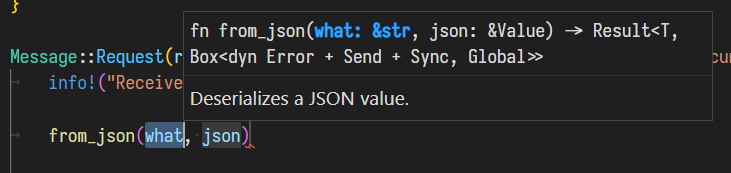
\includegraphics[width=1.00\textwidth]{resources/code_signature_help.png}
	\caption{Signature help in VS Code for Rust shows a pop-up with
	documentation as well as the signature of the callee, highlighting the
	parameter under cursor.}
\end{figure}

Auto-completion offers to fill in code as the programmer is typing, supports
ranking results based on their relevance, on both the server and the client
side, and can include a ``quick info'' description for each option. Signature
help shows parameter name and type information when calling a procedure, method,
or function. Formatting allows a language server to rewrite a document upon
request, for example to conform to a particular code style. The \acrshort{lsp}
formatting functionality can format either the entire document, a selected
range, or reactively an arbitrary part of the document as the user types.
Finally, symbol renaming performs a context-sensitive workspace-wide rename of a
given symbol.

\begin{figure}[t]\centering
	\begin{multicols}{3}
	\begin{enumerate}
		\item Inline Value
		\item Inline Value Refresh
		\item Moniker
		\item Completion Proposals \org
		\item Completion Item Resolve \org
		\item Publish Diagnostics
		\item Pull Diagnostics
		\item Signature Help \org
		\item Code Action
		\item Code Action Resolve
		\item Color Presentation
		\item Formatting \org
		\item Range Formatting \org
		\item On type Formatting \org
		\item Rename \org
		\item Prepare Rename
		\item Linked Editing Range
	\end{enumerate}
	\end{multicols}

	\caption{Coding language features in \acrshort{lsp} 3.17.}
	\label{fig:coding-requests}
\end{figure}

Later \acrshort{lsp} revisions added high-level features not universally
applicable to all programming languages. For instance, version 3.16 added
\emph{linked editing}, which some conforming implementations use to update
opening and closing \acrshort{xml} tags seamlessly without the user specifically
triggering a rename action. Version 3.17 introduced \emph{type hierarchy}
requests, relevant only to programming languages with subtyping. On the other
hand, more general facets of the protocol see creative use in unintended
contexts. One example is the use of lenses and special comments in the Haskell
Language Server project\cite{haskell_ls} to provide \acrshort{repl}-like
functionality. Another is the LT$_\text{E}$X Visual Studio Code
extension\cite{vscode_spellcheck}, which provides spell and grammar checking in
Markdown and \LaTeX{} documents, as well as in programming language comments.
Even though \acrshort{lsp} has no built-in support for extracting the comments
of a document or for spell checking in general, LT$_\text{E}$X achieves this
with a combination of non-\acrshort{lsp} \acrshort{api}s and by leveraging
\acrshort{lsp} diagnostics and code actions to provide suggested spellings.

\begin{figure}[h]\centering
	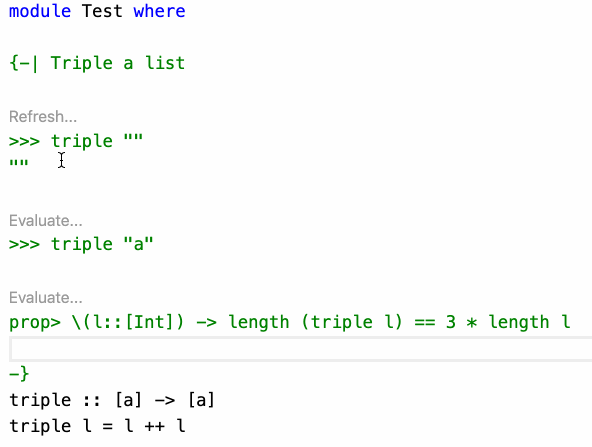
\includegraphics[height=0.3\textheight]{resources/code_haskell_repl.png}
	\caption{The Haskell Language Server project supports in-editor expression
	evaluation in comments prefixed with \texttt{>>>} and checking QuickCheck
	properties in comments starting with \texttt{prop>}.}
\end{figure}

\subsection{The state of the art}

Some of the best tooling in the \acrshort{lsp} ecosystem comes, somewhat
unsurprisingly, from Microsoft.

Projects which served as the de facto \acrshort{ide} integration for the given
language matured somewhat quicker than software that already had ample
competition.

\todo[inline]{the idea here is to compare "actual" language popularity
with the popularity of a corresponding language server.
We should see people preferring other tools for established technologies.}

We have chosen to exclude some technologies from this comparison. JavaScript,
TypeScript, CSS, and HTML support is built into VS Code and therefore does not
show up in VS Code marketplace statistics for installed language extensions.
SQL, while popular, has too many dialects to present a faithful picture through
the lens of extension installations alone. These technologies were in turn
filtered out from StackOverflow's list of most popular languages to highlight
the differences in ranking.

\todo[inline]{
	add the source
	% https://marketplace.visualstudio.com/search?target=VSCode&category=Programming%20Languages&sortBy=Installs
}

\begin{table}\centering
\caption{Popularity of programming languages among VS Code users and
StackOverflow's 2022 Developer survey\cite{stackoverflow_survey_2022}
respondents.}
\begin{tabular}{|r|c|c|}
	Rank & VS Code extension & Most popular programming and scripting languages
	\tabularnewline \hline
	1  & Python     & Python     \tabularnewline
	2  & C/C++      & Java       \tabularnewline
	3  & Java       & C\#        \tabularnewline
	4  & C\#        & C/C++      \tabularnewline
	5  & Go         & PHP        \tabularnewline
	6  & PHP        & PowerShell \tabularnewline
	7  & PowerShell & Go         \tabularnewline
	8  & Dart       & Rust       \tabularnewline
	9  & Ruby       & Dart       \tabularnewline
	10 & Rust       & Ruby       \tabularnewline
\end{tabular}
\end{table}

\todo[inline]{the whole thing above is kinda suspicious.
I'm not sure a comparison like that has a place in a language server thesis.}

%----------------------------------------%
\section{Lessons from the compiler world}
%----------------------------------------%

We have previously established how closely does the task of implementing
language servers relate to writing compilers. Let us expand on the possible
architectural similarities of the two kinds of language tools in this section.

\subsection{The pipeline}

Traditional compiler architectures build around a pipeline approach. The
compiler begins with a frontend, typically composed of a lexer\footnote{Although
the lexer/parser distinction is maintained, partly for historical reasons, in
many modern compilers, the jobs of lexers and parsers are conceptually
identical. These compositional algorithms transform input of one type (usually a
string) into output of another, verifying certain properties along the way.
Concretely, they match the input against some
grammar\footnotemark.}\footnotetext{A keen reader will note that without
restrictions on the \emph{class} of grammars, this statement makes the
description no more concrete.}, a parser, and a step of semantic analysis. The
second major part is the backend, a combination of an optimiser and a code
generator. The lexer ingests bytes of text, turning them into tokens for the
parser. The parser matches the tokens against the productions of a given
language's grammar, producing \acrlong{ast}s. Semantic analysis then verifies
that the parsed program adheres to the language's semantic restrictions. For
example, semantic analysis ensures that variables can only be referenced after
their declaration or definition, \texttt{break} statements can only appear in
the bodies of loops, and the program follows typing rules.

Is it the frontend's responsibility to identify and report user errors,
terminating the compiler pipeline as soon as it identifies invalid input. This
is a practical choice, since later stages of the compiler can assume the program
valid and not worry about possible errors. Furthermore, computation of the
backend stages would be wasted on invalid input anyway, as the compiler could
give no guarantees about the produced executable form\footnote{Whether that is
machine code in a platform-specific executable, bytecode for a virtual machine,
source code in the case of transpilers, or something else entirely.}.

One important step that typically happens on the frontend/backend boundary is
\emph{lowering}. This process turns the \acrshort{ast} obtained and validated by
previous stages into the compiler's \emph{\acrfull{ir}}. The \acrshort{ir}
represents a simplified language devoid of syntactical sugar and various
programmer-facing niceties. For example, various types of conditional
expressions are usually represented by a single \acrshort{ir}
instruction\footnote{Which may in fact conceptually be an instruction, or a node
of the \acrshort{ir} graph.}. Similarly, different forms of loops lower to a few
canonical translations. Freedoms in the source-level code style are eliminated
to make reasoning about the program further down the pipeline easier. Nested
expressions are flattened using short-lived local variables, often imposing an
evaluation order. Overall, \acrlong{ir}s tend to be semantically closer to the
target architecture.

After lowering, the backend takes over. The optimizer, if it is involved in the
compilation, iteratively transforms the \acrshort{ir} in a series of analysis
and rewriting steps that attempt to minimise certain cost functions\footnote{The
actual cost functions may vary based on what steps the optimizer takes. For
example, the metrics used for inlining can differ from heuristics consulted for
loop-invariant code motion.}. Optimization can sometimes cross the boundaries of
source-level code. That is, certain \acrshort{ir} programs do not have a
corresponding source program, because the lowering phase is not a surjective
mapping. This is a necessary freedom for eliminating overhead in implementations
of high-level programming languages, but makes mapping issues in the final
executable more difficult\footnote{Which is of major concern for debugging, and
consequently one of the primary reasons why native executable debuggers tend to
operate better on programs compiled with fewer optimizations.}.

Finally, the pipeline terminates in a code generation phase which emits the
final executable form. This step requires rewriting the \acrshort{ir} program in
order to fit the target constraints. The amount of work the compiler needs to do
in this last stage depends on the semantic differences between the structure of
the \acrlong{ir} and the target language. It could be as simple as writing the
\acrshort{ir} to an output file, if the intermediate and target languages
perfectly match. For conventional processor targets, however, code generation
necessitates at least instruction selection and register allocation, as well as
maintaining some level of conformance to standard calling conventions.

\subsubsection*{Born of necessity, sculpted for collaboration}

\todo[inline]{Figure out where did the pipeline design come from, how GCC
popularised it (I swear I heard that somewhere)}

\subsubsection*{Where the pipeline falls short}

In recent years, the feedback loop from writing code to executing it has gotten
shorter and shorter. The case for early feedback is simple: programmers want
results as soon as possible. Moreover, since the programmer typically uses the
compiler in an online fashion, changes to the source files tend to be small and
local. Compiling small changes in the source program often only requires small
changes to the output. With proper caching, most information can be reused from
previous runs of the compiler.

With semantic language support receiving more and more attention, the overlap
between compilers and interactive language tooling is only getting clearer. Both
classes of programs now need to maintain and incrementally update databases of
semantic information about the codebase in order to respond quickly to user
requests. With semantic information at hand, it is only natural for both classes
to integrate tightly with editors and development environments to provide
features reliant on high-level information. Both compilers and language servers
should be resilient to errors in the user input and continue processing as far
as is practical, for example to report semantic errors even in the presence of
syntactical issues. Just as with optimizers\todo{make sure we reference the
previous subsubsection here correctly}, reimplementing a lot of complicated
functionality is tiresome and unnecessary.

Unfortunately, the well-established pipeline approach to compiler construction
is, despite its many innovations, difficult to adapt to the modern incremental
workloads. The interfaces between stages do not share a principled, universal
structure, requiring each phase to implement its own variant of caching and
cache-invalidation. Running phases concurrently for independent sections of the
input program can be problematic, because older pipeline-based compilers often
rely on global variables\footnote{This is no fault of the architecture as a
whole, but it is an important practical consideration.}.

Conventional incremental compilers choose a granularity of input file,
compilation unit, or module, and often run several pipelines in parallel,
culminating in a sequential step that combines the constituent products into the
final executable. This approach achieves very short compilation and
recompilation times for many programs, but tends to produce suboptimal code,
since the optimiser can only see a subset of the code and is limited in
attempting whole-program optimisation and cross-module inlining. Nowadays,
linkers (the usual last step in the production of executables) counter this
downside with \acrfull{lto}, trading linking time for better quality code.
Running many pipelines in parallel also tends to increase the size of the
intermediate compilation artifacts, because dead code elimination cannot safely
remove unused definitions, possibly referenced by other compilation units.

\subsection{The pipeline as a sequence of queries}

With these new developments and performance constraints in mind, recent compiler
construction techniques put incremental computation at the centre of their
design. For example, Roslyn\footnote{This product is officially called \emph{The
.NET Compiler Platform SDK} but it is arguably better known under the Roslyn
codename.}, a collection of compilers and analysers for C\# and Visual Basic,
builds heavily on incremental computation. A Roslyn compiler takes centre stage
in a number of interactive and batch applications, maintaining a semantic model
of the codebase. Higher-level tools then query and update this model via several
\acrshort{api}s designed for static analysis, code refactoring, and other
use-cases\cite{roslyn_apis}\todo{what are some concrete applications that build
on these?}. The entire stack is optimised for interactive use. For example, the
parsers utilise a combination of persistent ``green'' \acrlong{ast}s and
transient ``red'' trees. The second, ephemeral type is built on-demand,
optimised for querying, and discarded with edits\cite{roslyn_red_green_trees},
while the ``green'' tree serves as the source of truth.

As more and more language tools interact with and rely on the compiler, compiler
authors find themselves adapting the pipelined architecture to emit additional
intermediate artifacts. If this evolution happens organically over long periods
of time and without a methodical approach, compiler codebases can degenerate
into clouds of complex, intertwined code.

A possible remedy is to adapt the pipeline architecture in ways that make it
simple to incrementalise and memoize its stages. The key insight is that the
pipeline is conceptually a collection of data-dependent queries. If we express
the compiler in the language of a general query engine, caching and incremental
computation features come for free. Propagating changes through the data
dependency graph is simple, and this change processing subsumes cache
invalidation. The interfaces between compiler queries effectively become
high-level \acrshort{api}s, with little extra work. These interfaces are shared
with other applications, making integration simpler and less error-prone than in
many traditional pipeline architectures, which maintain separate sets of
internal and external interfaces.

\subsubsection*{A functional approach}

Even though the traditional pipeline and its query-based reimagination are
conceptually close, their implementations are vastly different. Typical
compilers mutate global state during the course of a compilation. If any stages
produce additional data, they populate additional global maps and tables for
further passes to use. This can lead to subtle compiler bugs when compiler
passes are added, removed, or reordered. Mutable state is also an obstacle to
parallelism and makes it difficult to reason about where exactly in the pipeline
does one intermediate form change into another.

On the other hand, the query-based approach is inherently functional. Compiler
passes are ordered by their data dependencies and the amount of available
parallelism is limited only by the number of independent queries at a given
stage. A query-based compiler should avoid using mutable state, so that the
query engine can correctly propagate changes and update memoized
functions\footnote{Some hidden mutability may still be beneficial for
performance optimisations. For example, a hidden mutable map can serve as a
backing store for string interning. Naturally, the programmer needs to be
vigilant around any such places in the implementation and verify that the
introduced side-effects do not compromise correctness of the entire system.}.

\subsubsection*{Queries in the wild}

The Rust compiler was not originally built around a query system, but one has
been retrofitted into it, and major parts of the pipeline between
\texttt{rustc}'s high-level \acrshort{ir} and \acrshort{llvm} \acrshort{ir} are
now implemented as incremental interdependent queries.\todo{reference}

The Roslyn project\todo{add information from the GitHub discussions thread, once
available.}

\todo[inline]{include citations of the Sixten compiler, the rock library that
supports Sixten, the talk by Anders, and \texttt{rustc} queries. Also, build
systems a la carte, perhaps?}

%---------------%
\chapter{Design}
%---------------%

\todo[inline]{the design of the p4 language server, what it learned from
rust-analyzer, etc}

\begin{itemize}
	\item intention to do everything in-editor, Rust to WebAssembly
	\item cannot reuse the open-source frontend, not error-tolerant, difficult
	to work with, poor diagnostics
	\item needs to adapt to various backends and architectures easily
	\item open-source project, no point in keeping it closed, want to encourage
	contributions from the community
\end{itemize}

The high-level architecture of the \acrshort{p4} Analyzer project marks a
departure from conventional language server designs in that it primarily targets
WebAssembly and aims to run entirely within the Visual Studio Code editor. This
decision makes installation simpler for the end-user, cross-platform support
easier for the developers, and security policy conformance trivial for any
security teams involved.

The main mode of operation is thus as follows: the language server runs in a
WebAssembly worker of the \acrshort{p4} Analyzer VS Code extension. The
extension itself defines a simple TextMate\todo{reference} grammar specification
and serves as a thin client for the server. The main bulk of \acrshort{lsp}
functionality is delegated to the editor. VS Code forwards edits to open files
to the language server, which updates its model of the workspace. When VS Code
asks for completions, hover, diagnostics, or other features, the analyzer
recomputes necessary information on-demand and responds appropriately.

In addition to the WebAssembly executable, the \acrshort{p4} Analyzer project
also compiles to a native binary that executes in a standalone process and
communicates with an arbitrary \acrshort{lsp}-compliant client over a socket.
However, the standalone language server requires support for certain features
related to filesystem functionality that fall outside the protocol
specification. We will discuss these in-depth later\todo{make sure this is
indeed the case, put a reference here}.

%-----------------------------------------------%
\section{The \pdfacrshort{p4} Analyzer pipeline}
%-----------------------------------------------%

The first step in our pipeline is lexical analysis. Somewhat unconventionally,
our lexer produces tokens even for the preprocessor (i.e. it analyses
preprocessor directives). Our preprocessor then operates at the lexeme level,
rather than running separately as the first step. This requires a
reimplementation of the preprocessor, which is already necessitated by
fault-tolerance and WebAssembly support requirements anyway. On the upside, a
custom preprocessor simplifies tracking of source positions, which are crucial
for accurate diagnostics.

\subsection{Lexical analysis}

The \pfs specification defines a \acrshort{yacc}\todo{use a glossary entry
instead of an acronym}/Bison grammar for the language. However, this grammar has
several flaws.

For example, it reuses the \texttt{parserTypeDeclaration} non\-terminal in
\texttt{parserDeclaration}s but imposes extra restrictions: a parser declaration
may not be generic. This requires checking the child production outside the
grammar specification.

However, the primary issue is that the grammar design does not maintain a clean
separation between a parser and a lexer and requires these two components to
collaborate.

\begin{displayquote}
	\textit{The grammar is actually ambiguous, so the lexer and the parser must
	collaborate for parsing the language. In particular, the lexer must be able
	to distinguish two kinds of identifiers:}

	\begin{itemize}
		\item \textit{Type names previously introduced (\texttt{TYPE\_IDENTIFIER}
		tokens)}
		\item \textit{Regular identifiers (\texttt{IDENTIFIER} token)}
	\end{itemize}

	\textit{The parser has to use a symbol table to indicate to the lexer how to
	parse subsequent appearances of identifiers.}

	-- \citetitle{p416:v123:spec} \cite{p416:v123:spec}
\end{displayquote}

The specification goes on to show an example where the lexer output depends on
the parser state and mentions that the presented grammar ``\textit{has been heavily
influenced by limitations of the Bison parser generator tool.}''

The tight coupling between the lexer and the parser, as well as the decision to
remain in the confines of an outdated parser generator despite its many
drawbacks, are in our opinion examples of poor design for a language born in the
twenty-first century. We have elected not to follow this ambiguous grammar
specification in the \acrshort{p4} Analyzer project and instead build a pipeline
that is tolerant to invalid input to the fullest extent possible, while
accepting the same language.

Our lexer's task is to convert the input string into a stream of lexemes. The
lexer is a standalone finite state machine independent of any later stages in
the pipeline. It has a secondary output for reporting diagnostics, but this side
channel is write-only.

\subsubsection*{Error tolerance}

Error tolerance at the lexer level means proceeding with lexeme stream
generation despite nonsensical input. We emit a special error token whenever
such input is encountered. Additionally, the lexer validates numeric constants,
which can specify width, base, and signedness\todo{is this a word?}. These
properties could be out of bounds for a given literal. In these cases, the lexer
produces\todo{"should produce" language instead? since this is a design chapter,
wink wink?} a valid token anyway but logs an error-level diagnostic, which is
reported to the user once lexing completes.


\subsection{The preprocessor}

\pfs requires support for a preprocessor, very similar to the C preprocessor,
directly in the specification. However, it does not ask implementors to support
the entirety of \texttt{cpp}. Notably, only simple, parameter-less macros are
allowed. This is already enough to necessitate running the preprocessor before
starting the parser, however. Consider the code in
Listing~\ref{lst:p4pp}\todo{p4 syntax would be nice}. These examples show how
grammatically invalid code may become valid and vice versa, based only on the
right-hand sides of preprocessor macros.

An important consideration for a correct implementation of preprocessor
directives is their context-sensitive nature. Expressions for conditional
inclusion in directives \texttt{\#if}, \texttt{\#elif}, and \texttt{\#ifdef} are
themselves subject to macro substitution and thus have to be kept in plain text
or lexeme form until their evaluation.

One more thing to note here is the mechanism of document inclusion. Before
analysing a \pfs source file (at least to some degree), the full extent of its
dependencies is unknown and arbitrary. The language has no module system and
imposes no restriction on the paths a source file can include. This poses a
challenge for lexeme-level preprocessors, as a file needs to be lexed before it
can be included. To deal with this, a correct implementation should collect the
paths a source file can depend on, lex their contents, and include their lexemes
in the preprocessed lexeme stream. This is of particular note in our
implementation, as the collection of dependencies reports this dependency set to
the editor to set up filesystem-level watches. Subsequent edits to the
dependencies, or even to the dependency set itself, can be processed
incrementally.

\subsubsection*{Error tolerance}

Error tolerance in the preprocessor means reporting errors and warnings about
malformed input to the user while continuing to interpret directives in the
input stream on a best-effort basis. Mistakes in preprocessor directives come in
several flavours.

The directive itself may be malformed, either due to a typo in its name or a
problem in some of its arguments. The former case will simply be lexed as an
unrecognized directive and reported as such. It is possible to suggest fixes for
common typos to the user. A problem in the directive's argument or arguments
needs to be resolved based on its meaning. For example, an \texttt{\#include}
directive could point to a non-existent file, the preprocessor should then
report this error and proceed as if the file were not included. This is likely
to lead to further errors down the road, but without knowledge of the referenced
file's contents, it is the best a preprocessor can do.

Another class of errors is semantic and context-sensitive in nature: a directive
may be used in the incorrect context or missing where it is expected. For
example, a user may forget to add an \texttt{\#endif} directive, or include more
than one \texttt{\#else} directive for a condition. Unfortunately, guessing the
user's intention when faced with any syntactic or semantic problems in the input
is a tall order. No guarantees of optimality can be given, as is often the case
with similar heuristics. In the duplicate \texttt{\#else} problem, the
preprocessor could be reasonably expected to either skip over the first
\texttt{\#else}'s body, the second \texttt{\#else}'s body, or assume either of
the directives was inserted by accident and pretend it is not a part of the
input stream. We choose to skip the second \texttt{\#else}'s body in our design,
but other strategies are equally valid\todo{maybe it'd be better to look at some
data from users. But does this matter enough to bother with a study?}.

\begin{lstlisting}[
	caption={~\pfs preprocessor example},
	label=lst:p4pp,
	captionpos=t,
	tabsize=4,
	float,
	abovecaptionskip=-\medskipamount,
	belowcaptionskip=\medskipamount,
	language=c
]
#define op +
// #define op 2

#define paren )

header h {
	bit<1> field;
}

control pipe(inout h hdr) {
	Checksum16() ck;
	apply {
		// arithmetic expression could be invalid
		h.field = 1 op 3;
		// a parse without prior macro substitution would fail
		ck.clear( paren;
		// this would parse correctly, but macro substitution
		// will reveal a parse error
		ck.update(op);
	}
}
\end{lstlisting}


\subsection{The parser}

The next natural step in the pipeline is the act of finding the productions of a
\pfs grammar that match the preprocessed input program; parsing. While the steps
up to this point are fairly simplistic and efficient, parsing is a
resource-intensive process. A language server is expected to provide real-time
feedback to the developer, including auto-completion suggestions updated with
every keypress\todo{the lexer can identify a caret inside a (possibly
unfinished!) comment or string. Maybe we can learn from that for naive
lexer-based auto-completion?}. Low latency is crucial to the end-user and the
parser lies on every critical path from user input to high-level results shown
in the editor's interface. At the same time, a typical \pfs program is likely to
consist of a long prefix that does not change between edits and a
user-maintained suffix that changes frequently. This is because a \pfs program
usually begins with \texttt{\#include} directives referencing platform-specific
files with constants, error codes, \texttt{extern} definitions and other shared
code. These constraints and conditions are a very good fit for the field of
\emph{incremental parsing}.

An incremental parser aims to reuse previously computed information about the
input in response to small perturbations. Our parser specifically builds on
incremental packrat parsing\cite{dubroy2017incremental_packrat_parsing}, which
places few constraints on grammar design and is easy to implement in an
extensible manner.

Packrat parsing\cite{ford2002packrat} is a linear time algorithm for recognizing
productions of a \acrfull{peg}. It relies heavily on memoization to avoid costly
backtracking, at the expense of memory overhead.
\citeauthor{dubroy2017incremental_packrat_parsing} augment the packrat
memoization table to support incrementality. The result is a parser that is at
once simple, general, incremental, and efficient.

Our packrat parser conceptually handles \acrlong{peg}s\cite{ford2004parsing}, a
class of unambiguous grammars for context-free languages. \acrshort{peg}s are
syntactically similar to \acrlong{cfg}s. However, the choice operator in
\acrshort{cfg}s is ambiguous, whereas \acrshort{peg}s use ordered choice, which
greedily attempts to match alternatives in order. The right-hand side of a
\acrlong{peg} rule can also contain predicates, which attempt to match without
consuming input. Predicates are useful for positive and negative look\-ahead.

Our design differentiates between a generic parser library and a parser built on
it. Grammars are defined using a small \acrshort{dsl} implemented with Rust's
declarative macros. An example can be seen in
Listing~\ref{lst:grammar-dsl-example}. The~\texttt{grammar!} macro expands to a
data structure representing the grammar itself. This structure can be passed to
a smart constructor, which validates the grammar\footnote{Ensuring all
referenced non-terminals are in fact defined, and that \texttt{start} is
present.} and returns a parser. The implementation interprets the grammar
\acrshort{dsl} at runtime.

If future testing and development necessitate optimization of the parser, there
is room to build a parser compiler for the \acrshort{dsl} and generate a more
efficient solution from the same grammar. Procedural Rust macros\footnote{While
declarative macros can only perform a very restricted set of rewriting
operations on token trees, procedural macros can run arbitrary Rust code during
expansion.} could take care of integrating the parser compiler into the build
process.

\subsubsection*{Incremental updates}

Since the parser is required to process incremental updates to the input
sequence, it is not simply a function from a sequence of tokens to a parse tree.
Rather, the parser takes a reference to a read-write lock of the input. It
defines an \texttt{apply\_edit} method that acquires a write lock of the input
sequence, applies the change, invalidates relevant entries in the memoization
table, and releases the lock.

To initiate parsing, the user invokes the \texttt{\_match} method\footnote{Named
as such because \texttt{match} is a Rust keyword.}, which acquires a read lock
on the input for the duration of parsing.


\begin{lstlisting}[
	caption={~Example grammar in our \acrshort{dsl}.},
	label=lst:grammar-dsl-example,
	captionpos=t,
	tabsize=4,
	float,
	abovecaptionskip=-\medskipamount,
	belowcaptionskip=\medskipamount,
	language=c
]
grammar! {
	// The initial non-terminal is called `start`
	start => p4program;
	// The postfix `rep` operator corresponds to Kleene star
	ws => whitespace rep;
	// Non-terminals can expand to terminals by wrapping the terminal in
	// parentheses
	whitespace => (Token::Whitespace);

	// The right hand side can also be a sequence separated by commas
	p4program => ws, top_level_decls, ws;
	// ...or a choice separated by pipes
	top_level_decls =>
		top_level_decls_rep | top_level_decls_end | nothing;
	top_level_decls_rep => top_level_decl, ws, top_level_decls;
	top_level_decls_end => (Token::Semicolon);

	direction => dir_in | dir_out | dir_inout;
	// Rules can also match tokens against an arbitrary Rust pattern,
	// which is useful for identifying soft keywords
	dir_in    => { Token::Identifier(i) if i == "in" };
	dir_out   => { Token::Identifier(i) if i == "out" };
	dir_inout => { Token::Identifier(i) if i == "inout" };
}
\end{lstlisting}


\subsubsection*{Error reporting}

Error handling in parsing is far more nuanced than in any of the previous steps,
which is not surprising, considering the relative complexity of the languages
that the individual steps recognize and process. A good parser should attempt to
provide as much feedback as possible to the user, even when faced with
unexpected tokens. It is not enough to simply stop at the first error, and it is
not enough to be imprecise about the locations of problems in the source file.
Both of these considerations pose some challenges.

The desire to continue parsing malformed input to provide feedback to the
developer has a long history\cite{graham1975practical}. Error recovery has been
studied at length in \acrlong{peg}s as well\cite{redziejowski2009mouse,
maidl2013exception, demedeiros2016parsing, demedeiros2018syntax,
demedeiros2020automatic}. The \acrshort{peg} case is interesting, because a
packrat parser relies on failures to guide choice selection. By the time a
parsing failure propagates to the starting non-terminal, the information about
the context that led to it is lost.

Specifically, when encountering unexpected input, a packrat parser unwinds the
stack to a ``calling'' ordered choice operator, and attempts to parse the next
alternative. The next alternative is likely the wrong choice, however. The
recently failed alternative should have matched, but encountered invalid input.
Thus, many other alternatives may fail before an error eventually propagates to
the user. The end result is that the programmer receives an unhelpful error
message that could potentially come from a position many tokens before the
actual problem's origin. This specific challenge has a popular practical
solution in the form of the \emph{farthest failure
heuristic}\cite{ford2002packrat_non_func}. It is based on the observation that
the alternative that should have matched will probably process the longest
prefix of the token stream.

While the farthest failure heuristic addresses the location problem in many
practical situations, it is not a general solution. Worse, the imprecise error
reporting of \acrshort{peg}s has other implications as well. Notably, a common
consideration for error messages is the suggestion of expected tokens to the
user, to provide a rudimentary selection of possible fixes. However, the
compounding failures of \acrshort{peg} choice operators grow the set of expected
tokens, which makes the suggestions in error messages irrelevant.

Intuitively, the problem with \acrshort{peg} error reporting is that
non-terminals deeper down the parse tree have no way of distinguishing between
an error in the input that will ultimately cause the overall parse to fail, and
an error that can be recovered from in an ordered choice operator higher up.

To address this problem, \citeauthor{maidl2013exception} conservatively extended
the \acrshort{peg} formalism with \emph{error labels}\cite{maidl2013exception}.
Error labels semantically\footnote{In the sense that we are adding semantic
information to the process that analyzes syntax.} stand for errors that a
grammar rule can raise when encountering unexpected input. This differentiates
errors caused by nonsensical input from benign parse failures, and thus solves
the problem of accurate error reporting in \acrlong{peg}s\footnote{At the
expense of extensive manual annotations of the grammar. See
\cite{demedeiros2020automatic} for a possible remedy.}. The extension comprises
several components:

\todo[inline]{we actually do want a full syntax for \acrlong{peg}s}

\begin{itemize}
	\item The \acrlong{peg} is extended with a finite set of labels $L$.
	\item A special failure label \texttt{fail}, $\texttt{fail} \not \in L$, is
	also added to the grammar. This label indicates a benign failure that can be
	caught by the ordered choice operator.
	\item The grammar of \acrlong{peg} right-hand sides is enriched with the
	\texttt{throw} operator, which takes a label $l \in L$ as an argument. An
	error thrown by \texttt{throw} cannot be caught by ordered choice and thus
	indicates a parse error that should be immediately reported to the user.
	\item Rules are modified to include instances of the \texttt{throw}
	operator.
\end{itemize}

The error label extension is reminiscent of exception handling in ordinary
programming languages, and indeed was originally modelled after it, complete
with an extension of ordered choice playing (the role of)
\texttt{catch}\cite{demedeiros2016parsing}. However, the \texttt{catch}-like
mechanism is not necessary for error recovery, so we will not discuss it
further.

Error labels returned by the parsing process can be mapped to readable error
messages. Because the parsing process terminates early, the set of expected
tokens is kept accurate. In addition, having a single, obvious point of failure
also makes location tracking trivial.

\subsubsection*{Tracking source locations}

However, our setting complicates location tracking. Source locations are an
important consideration for any incremental parser. A naive implementation, that
includes the source locations in the parse tree, leads to a linear amount of
work per edit, as the parser must recompute the source location of every node.
This would largely defeat the purpose of incremental parsing. At the same time,
source locations are important for features such as go to definition, or
diagnostics generated by semantic analysis in subsequent processing steps. While
we could keep all positions relative,

Fortunately, the nature of the incremental parsing approach of
\citeauthor{dubroy2017incremental_packrat_parsing} permits an interesting hybrid
between

\todo[inline]{mention that we can trade off memory for speed in the preprocessor
by controlling memoization in a fine-grained manner using Salsa.}

\todo[inline]{ example of complex preprocessor logic
	% https://github.com/Princeton-Cabernet/p4-projects/blob/10a4b9ce25b725b5269ba857470f63c96f82c645/AES.p4app/AES.p4#L18
}


\listoftodos[Work in progress]
